% ================= 3. THIẾT KẾ GIAO DIỆN =================
\section{Thiết kế giao diện}

\begin{frame}{Nguyên tắc thiết kế và bố cục chuẩn của mọi Form}
\begin{columns}[T]
\column{0.44\textwidth}
\centering
\begin{tikzpicture}[font=\tiny]
\node[frm=white, minimum width=6.0cm, minimum height=4.4cm] (f) at (0,0) {};
\node[fill=navy!10, minimum width=6.0cm, minimum height=0.35cm, anchor=north] at (f.north) {};
\node[anchor=west] at ($(f.north west)+(0.1,-0.18)$) {Tiêu đề Form};
\node[frm=tvA!10, minimum width=5.7cm, minimum height=0.75cm, anchor=north] (flt) at ($(f.north)+(0,-0.5)$) {\textbf{1. Thanh lọc / nhập}: Label + TextBox/ComboBox + nút Search};
\node[frm=white, minimum width=5.7cm, minimum height=2.0cm, anchor=north] (grid) at ($(flt.south)+(0,-0.12)$) {};
\foreach \y in {0.45,0.15,-0.15,-0.45}{\draw[black!25] ($(grid.west)+(0,\y)$) -- ($(grid.east)+(0,\y)$);}
\node[fill=white] at (grid.center) {\textbf{2. Lưới \code{DataGridView}} -- chỉ đọc, chọn cả dòng};
\node[frm=tvB!10, minimum width=5.7cm, minimum height=0.55cm, anchor=north] (act) at ($(grid.south)+(0,-0.12)$) {\textbf{3. Nút nghiệp vụ} (trái) \hspace{1.5cm} \textbf{Close/Exit} (phải)};
\end{tikzpicture}

\vspace{1mm}
{\tiny Form danh sách (\code{TicketListForm}, \code{CustomerListForm}, \code{BookingForm}) theo 3 vùng trên; Form nhập/chi tiết dùng lưới nhãn--ô 2 cột, nút Save/Cancel góc dưới phải.\par}
\column{0.54\textwidth}
\scriptsize
\begin{itemize}
  \item \textbf{Một Main Shell} (\code{MainForm}): menu Tickets / Customers / Bookings / Reports / Account, thanh trạng thái sẽ nhận thông báo từ \code{UiNotificationObserver} (GĐ 4; hiện observer còn thân rỗng).
  \item \textbf{Menu theo vai trò}: Reports chỉ Manager thấy; Record Survey chỉ Agent thấy; nút Auto Assign/Assign ẩn với Agent. Quyền vẫn được kiểm tra lại ở tầng nghiệp vụ.
  \item \textbf{Form chỉ gọi Service}, không chứa quy tắc nghiệp vụ; mọi handler bọc trong \code{ErrorHandler.Run()} $\to$ lỗi nghiệp vụ hiện hộp thoại cảnh báo, lỗi khác ghi log.
  \item Form con mở dạng hộp thoại (\code{ShowDialog}); \code{*.Designer.cs} chỉ tạo control nên mở được bằng Designer của Visual Studio.
  \item \textbf{Quy ước tên control}: \code{txt}, \code{cbo}, \code{btn}, \code{dgv}, \code{col}, \code{num}, \code{dtp}, \code{lbl}, \code{mnu}, \code{sts}.
  \item Ngày giờ hiển thị \code{yyyy-MM-dd HH:mm} (ngày đặt phòng: \code{yyyy-MM-dd}); tiền USD 2 chữ số thập phân; chữ trên giao diện bằng tiếng Anh.
\end{itemize}
\end{columns}
\end{frame}

\begin{frame}{Sơ đồ điều hướng màn hình}
\centering
\resizebox{\textwidth}{!}{%
\begin{tikzpicture}[
  f/.style={draw=black!55, fill=white, rounded corners=2pt, font=\scriptsize, minimum width=2.7cm, minimum height=0.55cm, align=center},
  m/.style={draw=navy, fill=navy!12, rounded corners=2pt, font=\scriptsize\bfseries, minimum width=2.7cm, minimum height=0.55cm},
  a/.style={-{Stealth[length=1.8mm]}, draw=black!60}]
\node[f, fill=common!15] (login) at (-3.6,3.2) {\code{LoginForm}};
\node[m, fill=navy, text=white, minimum width=15.4cm] (main) at (6.3,3.2) {\code{MainForm} -- Main Shell (menu + thanh trạng thái)};
\draw[a] (login) -- node[above,font=\tiny]{đăng nhập} (main);
\draw[a] (main.north west) to[out=150,in=60] node[above,font=\tiny]{Log Out} (login.north);
\foreach \x/\n/\t in {0/mt/Tickets, 3.15/mc/Customers, 6.3/mb/Bookings, 9.45/mr/Reports, 12.6/ma/Account}{
  \node[m] (\n) at (\x,2.0) {\t}; \draw[a] (main.south -| \n) -- (\n);}
\node[f, fill=tvA!10] (tl) at (0,0.9) {\code{TicketListForm}\\{\tiny UC3, UC5 \ [M, A]}};
\node[f, fill=tvA!10] (te) at (0,-0.4) {\code{TicketEditForm}\\{\tiny UC2 \ [M, A]}};
\node[f, fill=tvA!10] (td) at (0,-1.7) {\code{TicketDetailForm}\\{\tiny UC4 \ [A: Start/Resolve; M: Close/Reopen]}};
\node[f, fill=tvB!10] (cl) at (3.15,0.9) {\code{CustomerListForm}\\{\tiny UC6 \ [M, A]}};
\node[f, fill=tvB!10] (ce) at (3.15,-0.4) {\code{CustomerEditForm}\\{\tiny UC6 \ [M, A]}};
\node[f, fill=tvB!10] (ch) at (3.15,-1.7) {\code{CustomerHistoryForm}\\{\tiny UC9 \ [M, A]}};
\node[f, fill=tvB!10] (sf) at (3.15,-3.0) {\code{SurveyForm}\\{\tiny UC8 \ [chỉ A]}};
\node[f, fill=tvB!10] (bf) at (6.3,0.9) {\code{BookingForm}\\{\tiny UC7 \ [M, A]}};
\node[f, fill=tvB!10] (rf) at (9.45,0.9) {\code{ReportForm}\\{\tiny UC10 \ [chỉ M]}};
\node[f] (lo) at (12.6,0.9) {Log Out / Exit};
\foreach \a/\b in {mt/tl, mc/cl, mb/bf, mr/rf, ma/lo}{\draw[a] (\a) -- (\b);}
\draw[a] (tl.west) -- ++(-0.35,0) |- node[pos=0.75,above,font=\tiny]{New} (te.west);
\draw[a] (tl.west) -- ++(-0.35,0) |- node[pos=0.8,above,font=\tiny]{Details} (td.west);
\draw[a] (cl.east) -- ++(0.3,0) |- node[pos=0.75,above,font=\tiny]{New/Edit} (ce.east);
\draw[a] (cl.east) -- ++(0.3,0) |- node[pos=0.8,above,font=\tiny]{History} (ch.east);
\draw[a] (mc.west) -- ++(-0.2,0) |- (sf.west);
\node[font=\scriptsize, text width=7.6cm, align=left, anchor=north west] at (5.3,-0.6) {Menu cũng mở thẳng: New Ticket, Ticket Details, New Customer, Interaction History, Record Survey.\\[2pt]
\textcolor{tvA}{$\blacksquare$} Form TV1 \quad \textcolor{tvB}{$\blacksquare$} Form TV2 \quad [M] Manager, [A] Agent};
\end{tikzpicture}}
\end{frame}

\begin{frame}{Màn hình đăng nhập và Main Shell}
\begin{columns}[c]
\column{0.38\textwidth}
\centering
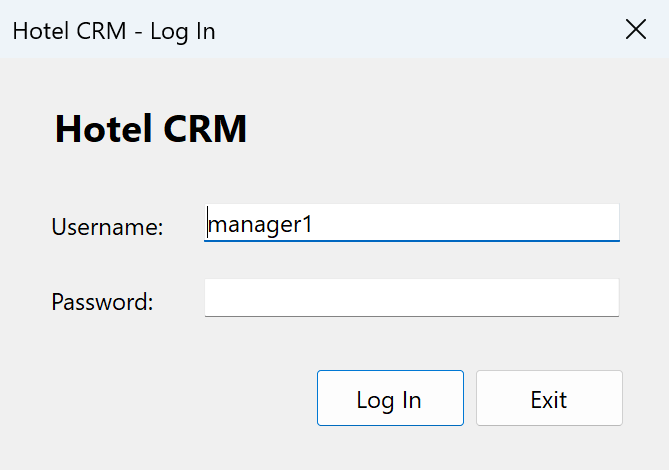
\includegraphics[width=\linewidth]{img/01-login.png}\\[1mm]
{\scriptsize \code{LoginForm}: sai tài khoản/mật khẩu $\to$ \code{Employee.EnsureLoginValid()} ném lỗi; mật khẩu so bằng PBKDF2.\par}
\column{0.6\textwidth}
\centering
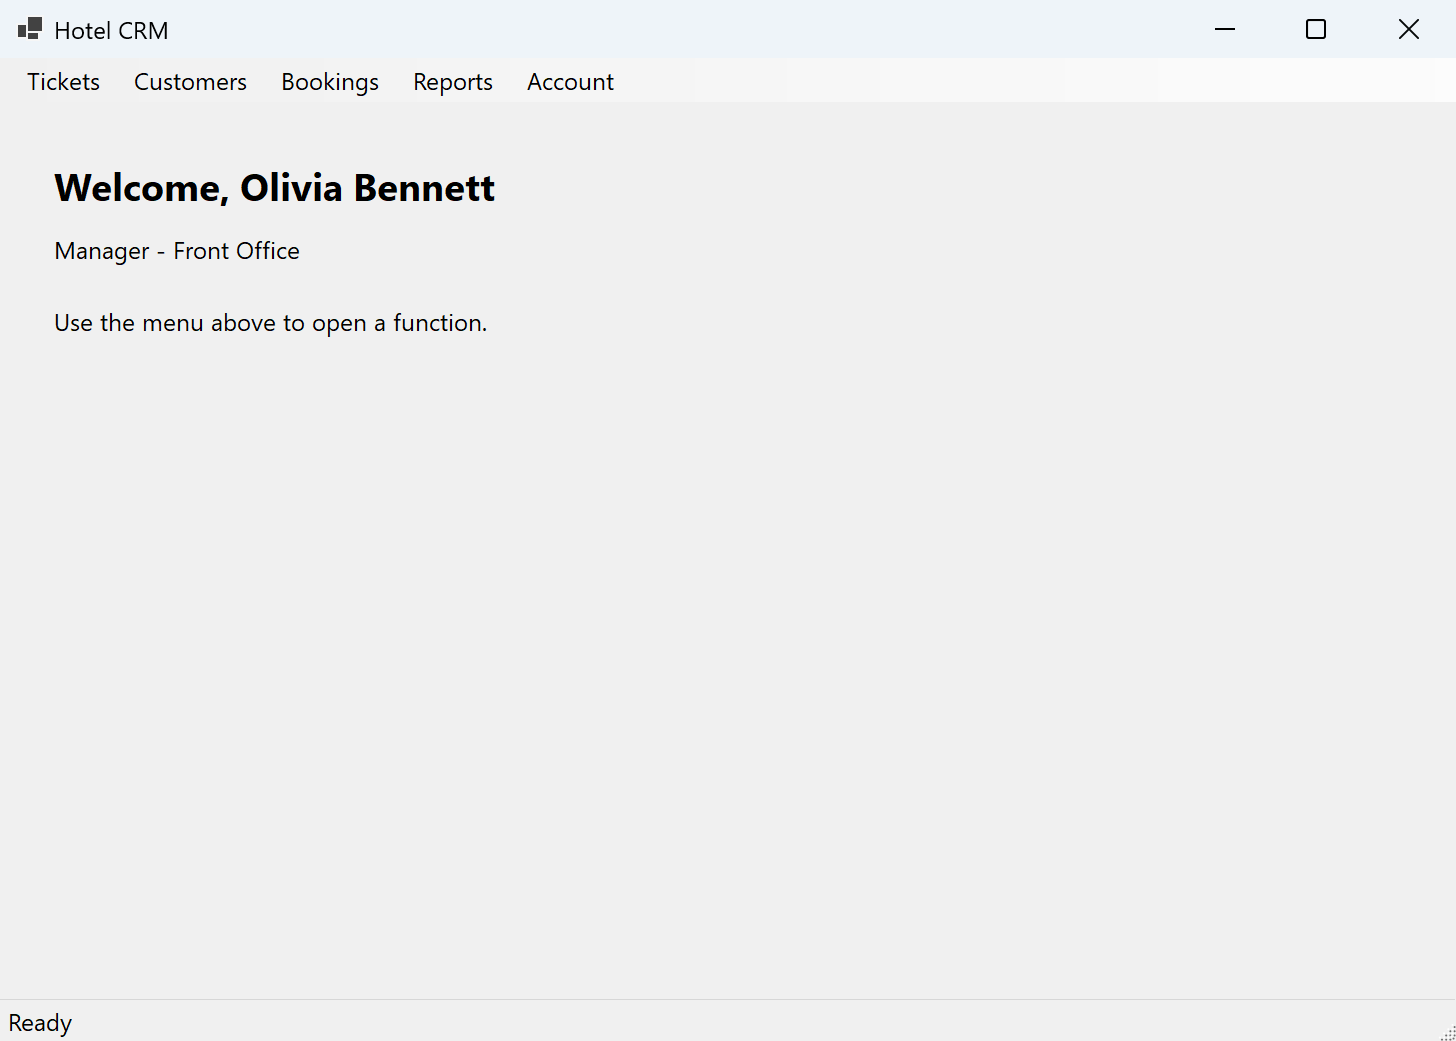
\includegraphics[width=\linewidth]{img/02-main.png}\\[1mm]
{\scriptsize \code{MainForm} của Manager: thấy menu Reports; Agent thì thấy Record Survey. Thanh trạng thái ``Ready'' sẽ hiện thông báo đổi trạng thái ticket ở GĐ 4.\par}
\end{columns}
\end{frame}

\begin{frame}{Phân hệ Ticket (TV1) -- \code{TicketListForm} (UC3, UC5)}
\begin{columns}[c]
\column{0.64\textwidth}
\centering
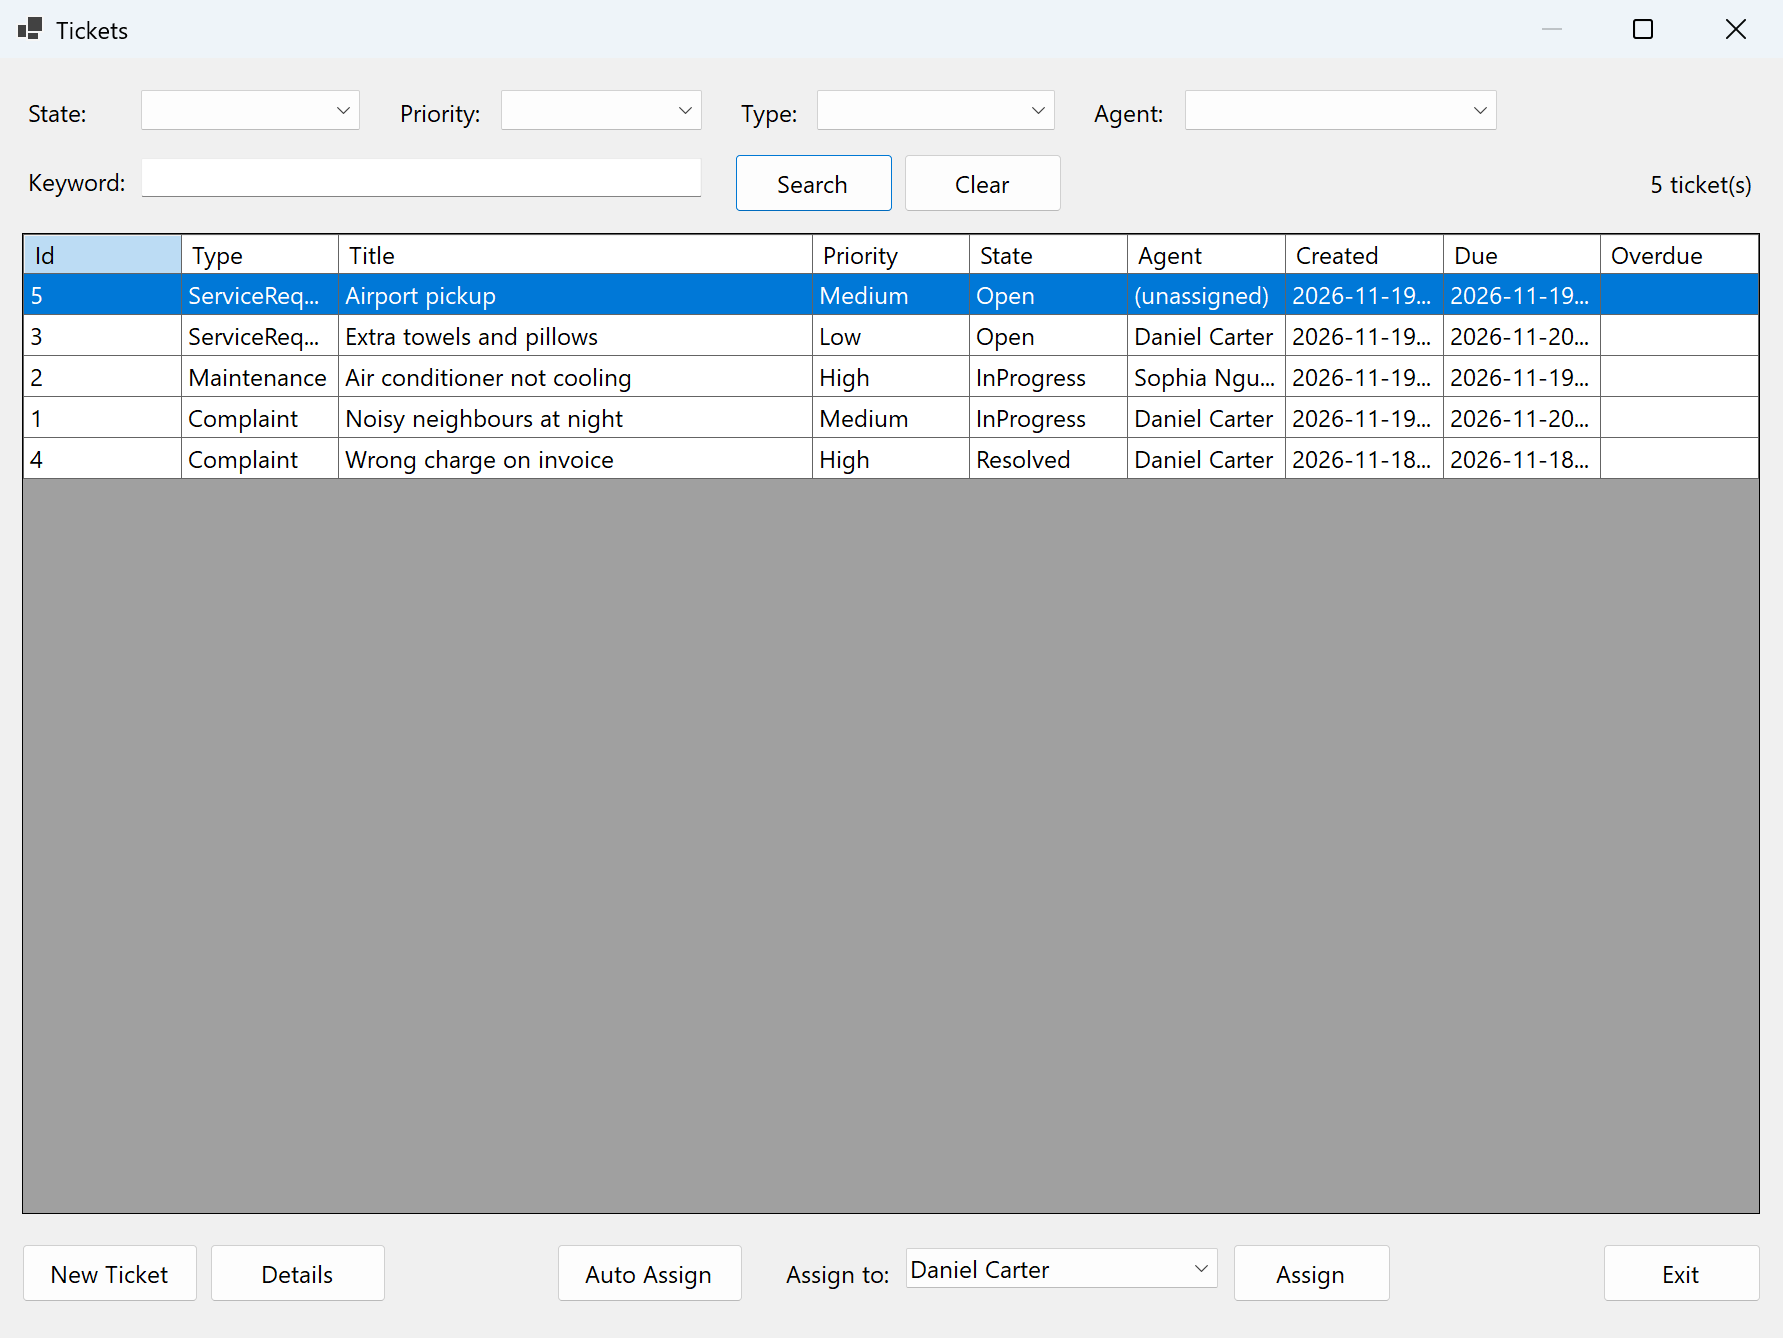
\includegraphics[width=\linewidth]{img/03-ticket-list.png}
\column{0.34\textwidth}
\scriptsize
\begin{itemize}
  \item \textbf{Lọc 5 tiêu chí}: State, Priority, Type, Agent, từ khóa tiêu đề $\to$ \code{TicketService.Search()}.
  \item Lưới: Id, Type, Title, Priority, State, Agent, Created, \textbf{Due} (hạn SLA), \textbf{Overdue}.
  \item \textbf{Auto Assign} $\to$ \code{AutoAssign()} (Strategy); \textbf{Assign to} + \textbf{Assign} $\to$ \code{AssignManually()}. Hai nút ẩn với Agent.
  \item \textbf{New Ticket}, \textbf{Details} mở Form con; đóng Form con thì nạp lại lưới.
\end{itemize}
\end{columns}
\end{frame}

\begin{frame}{Phân hệ Ticket (TV1) -- tạo ticket (UC2) và xử lý ticket (UC4)}
\begin{columns}[c]
\column{0.42\textwidth}
\centering
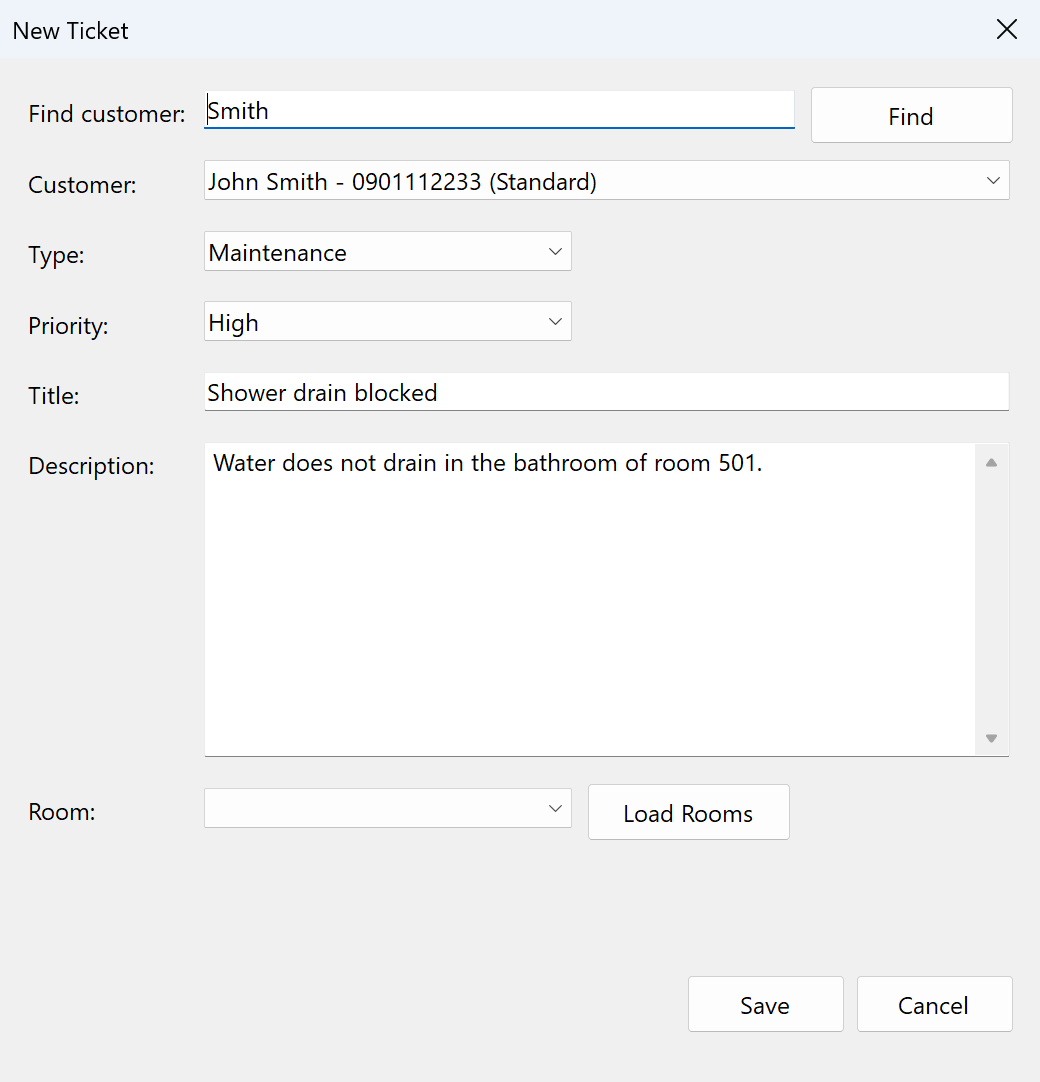
\includegraphics[height=0.6\textheight]{img/04-ticket-edit.png}\\[1mm]
{\tiny \code{TicketEditForm}: tìm khách $\to$ chọn loại, mức độ $\to$ Save. Loại Maintenance bắt buộc chọn phòng; Load Rooms chỉ trả phòng khách đang ở.\par}
\column{0.56\textwidth}
\centering
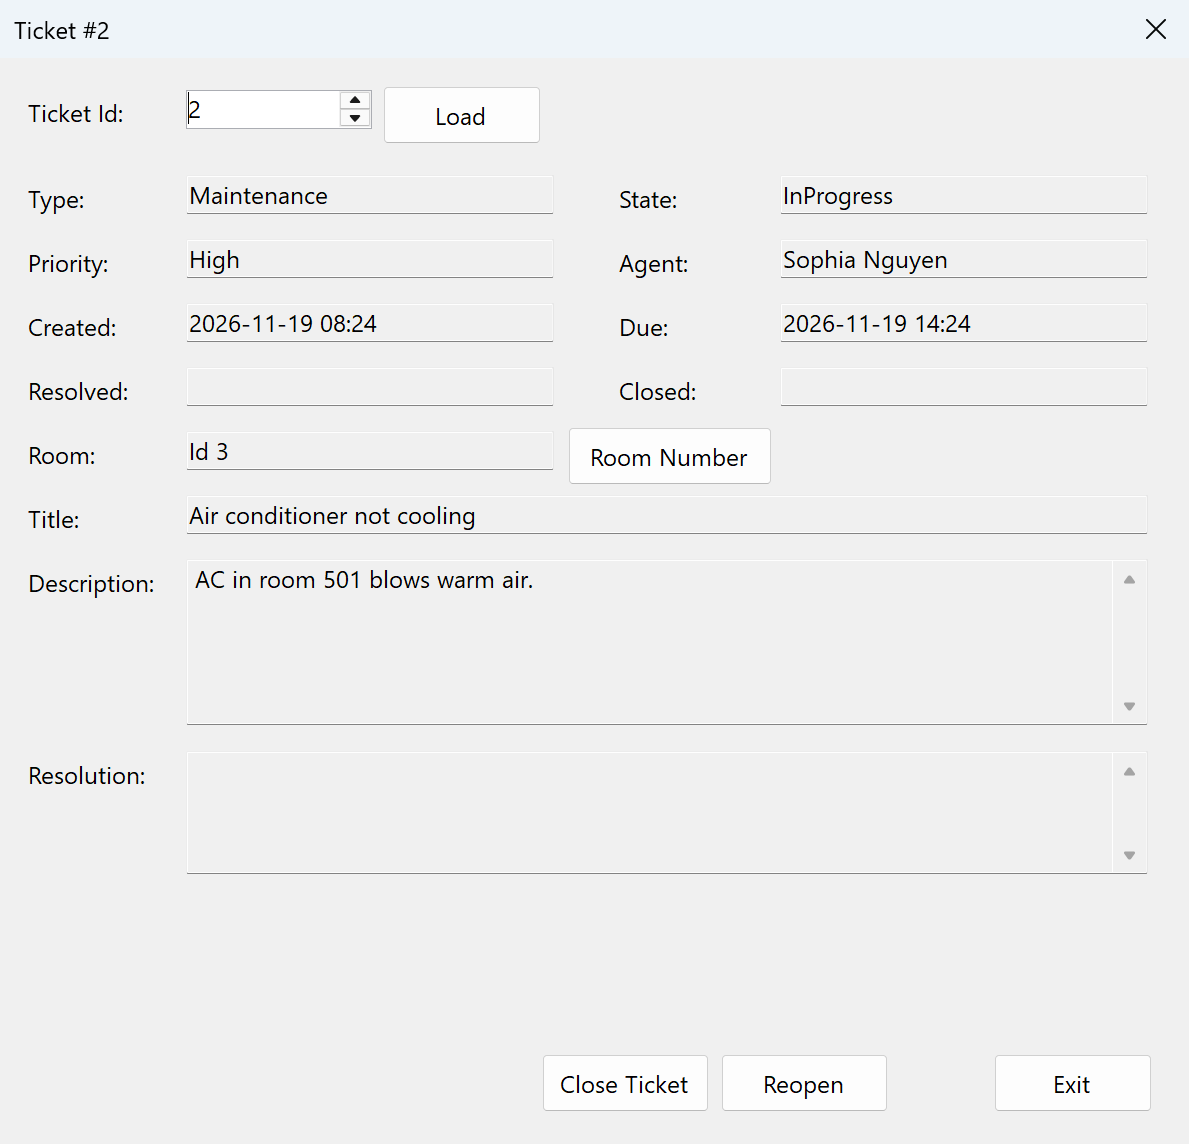
\includegraphics[height=0.6\textheight]{img/05-ticket-detail.png}\\[1mm]
{\tiny \code{TicketDetailForm}: đủ trường của phiếu theo dõi (BM2). Agent thấy Start/Resolve (chỉ Agent được giao mới làm được, \code{EnsureAssignedTo()} chặn người khác), Manager thấy Close Ticket/Reopen; State quyết định thao tác nào hợp lệ.\par}
\end{columns}
\end{frame}

\begin{frame}{Phân hệ Khách hàng (TV2) -- \code{CustomerListForm}, \code{CustomerEditForm} (UC6)}
\begin{columns}[c]
\column{0.58\textwidth}
\centering
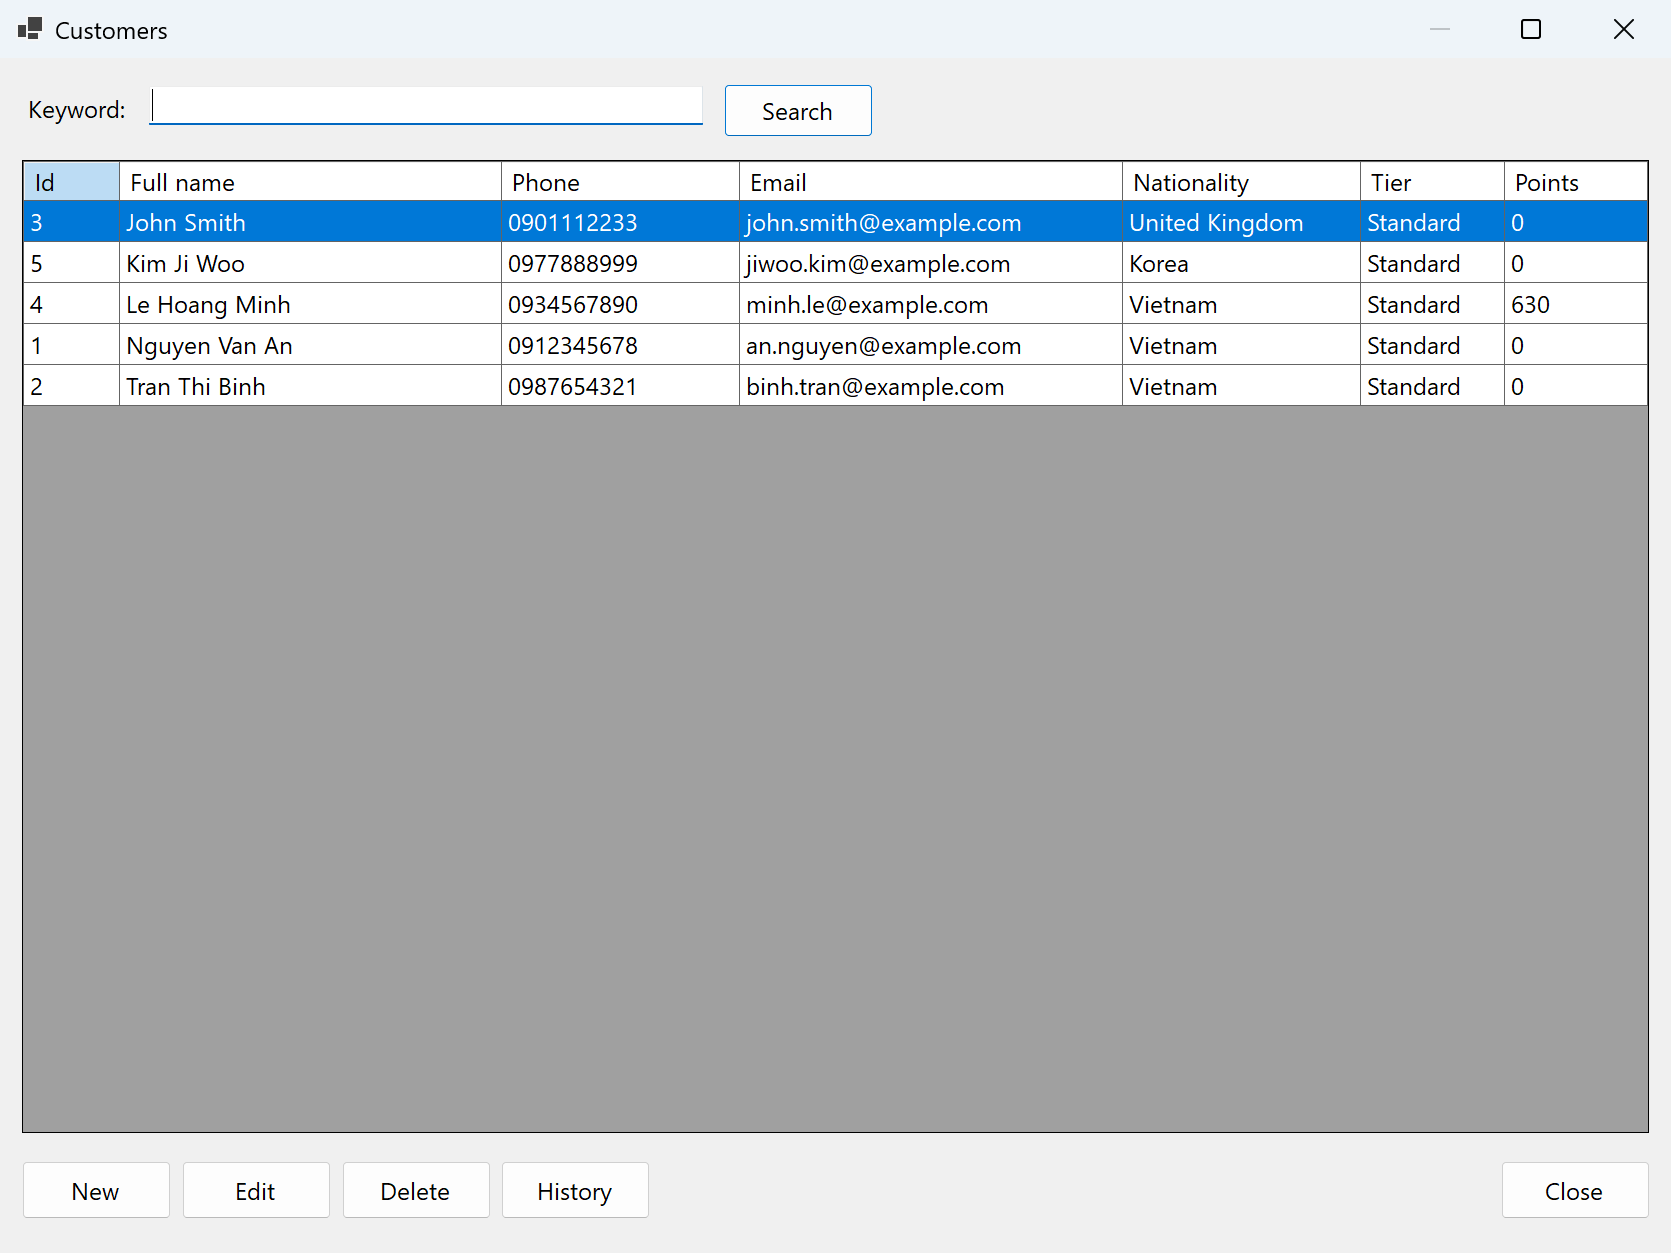
\includegraphics[width=\linewidth]{img/06-customer-list.png}\\[1mm]
{\tiny Tìm theo tên/SĐT/email; lưới hiện hạng (Tier) và điểm (Points). Delete bị chặn nếu khách còn ticket chưa đóng hoặc đã có booking.\par}
\column{0.4\textwidth}
\centering
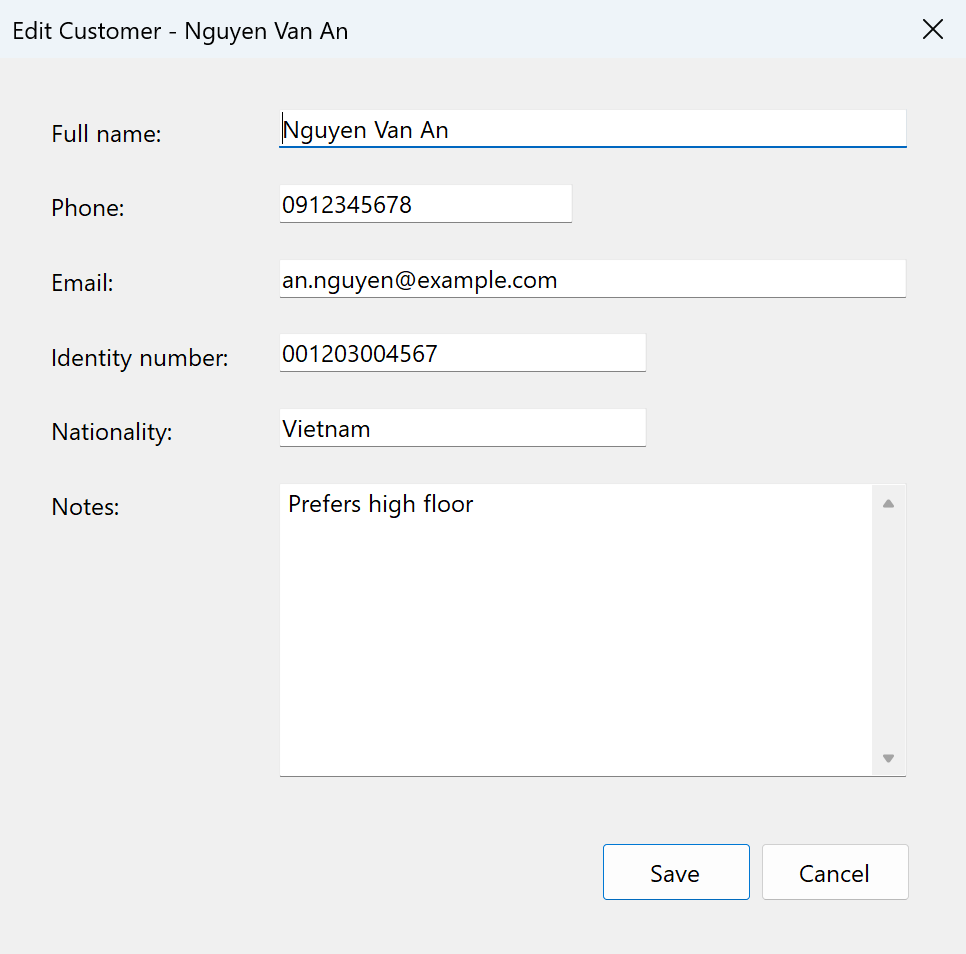
\includegraphics[width=0.92\linewidth]{img/07-customer-edit.png}\\[1mm]
{\tiny Ô nhập theo hồ sơ khách (BM3). Sai định dạng hoặc trùng SĐT/email $\to$ hộp thoại cảnh báo, không lưu.\par}
\end{columns}
\end{frame}

\begin{frame}{Phân hệ Lưu trú (TV2) -- \code{BookingForm} (UC7)}
\begin{columns}[c]
\column{0.64\textwidth}
\centering
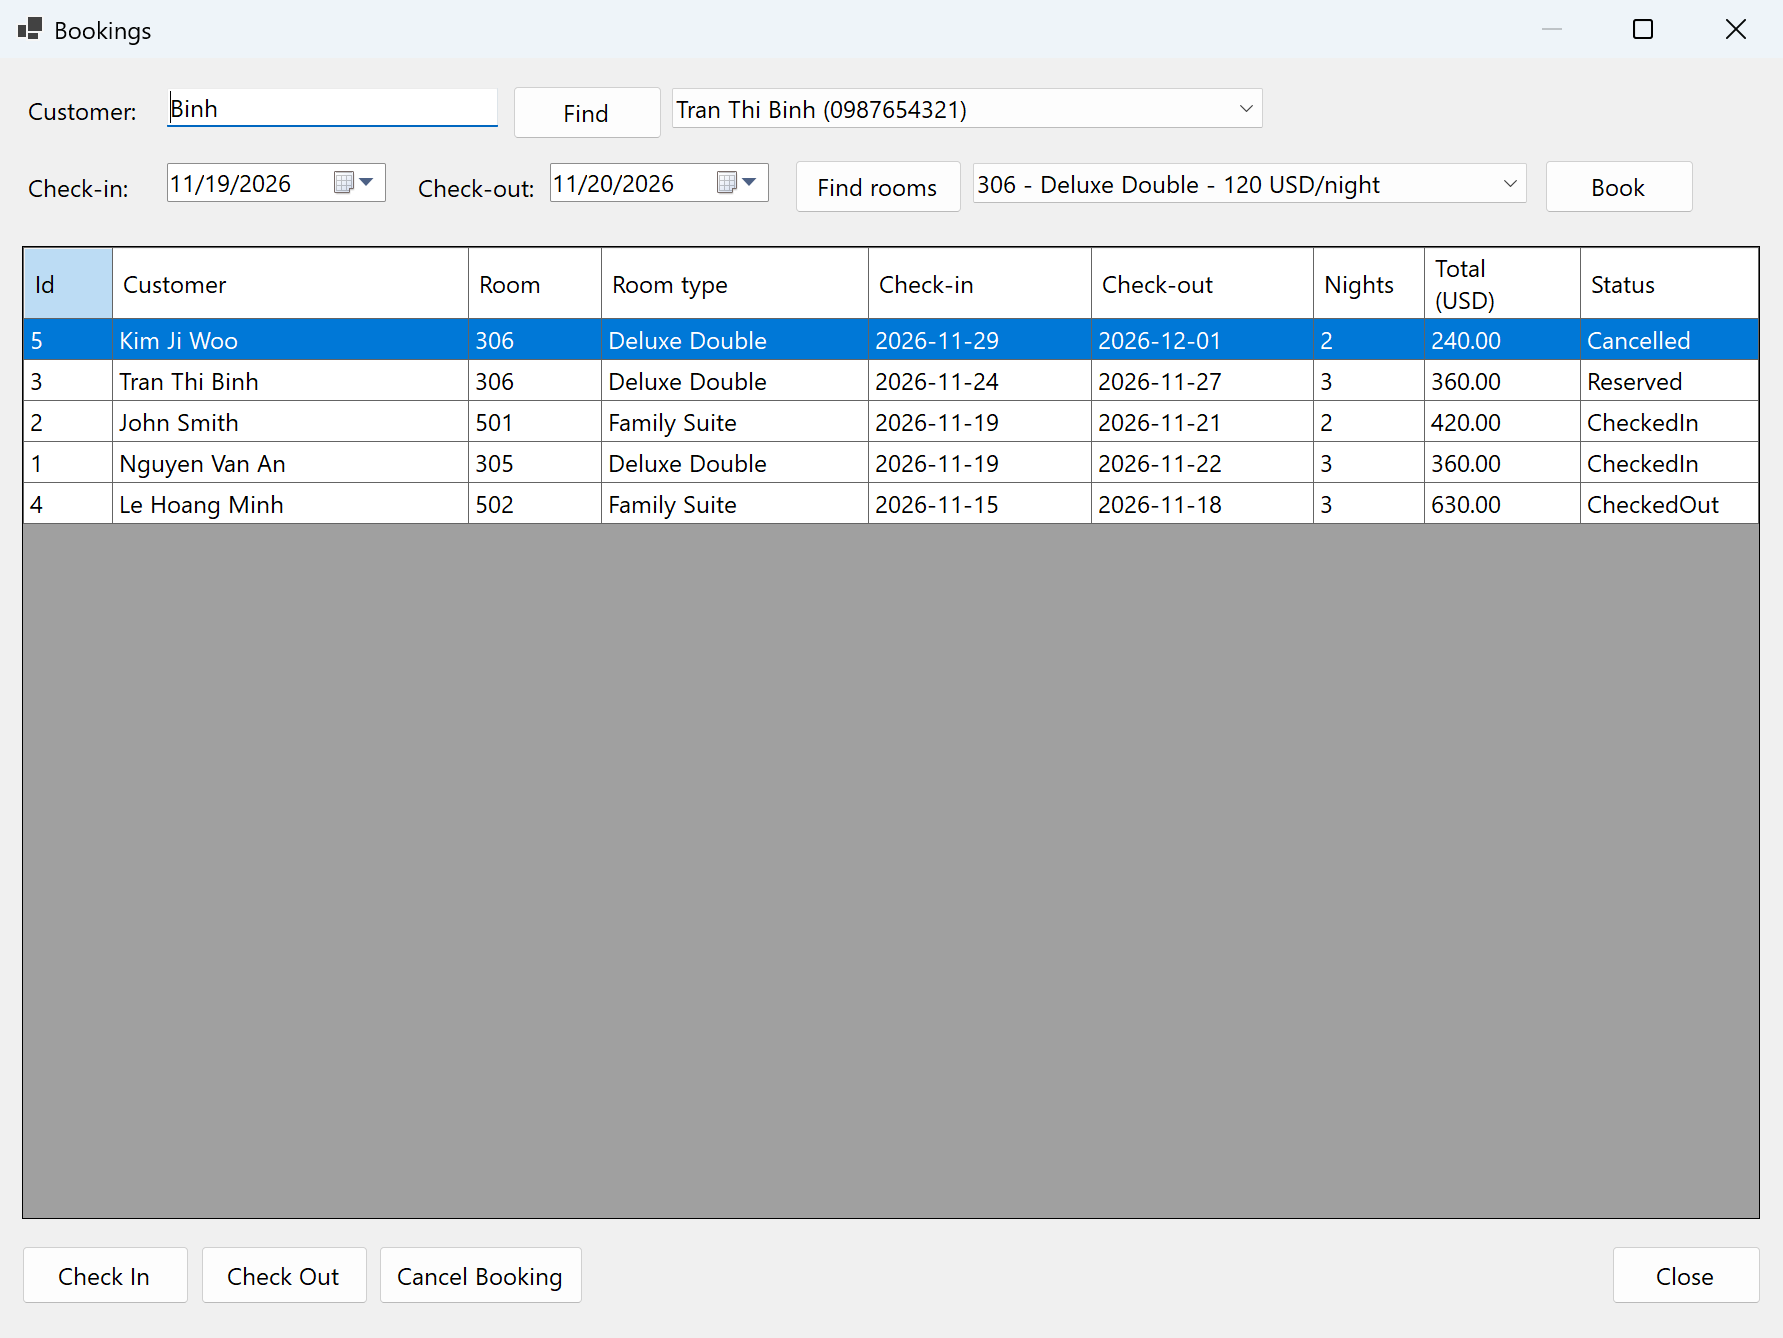
\includegraphics[width=\linewidth]{img/08-booking.png}
\column{0.34\textwidth}
\scriptsize
\begin{itemize}
  \item Dòng 1: tìm khách (\code{txtCustomerKeyword} $\to$ \code{cboCustomer}).
  \item Dòng 2: chọn ngày nhận/trả $\to$ \textbf{Find rooms} chỉ liệt kê phòng trống, sắp theo tầng $\to$ \textbf{Book}.
  \item Lưới: số đêm, \textbf{Total (USD)} = đêm $\times$ giá, trạng thái Reserved / CheckedIn / CheckedOut / Cancelled.
  \item \textbf{Check In}, \textbf{Check Out} (cộng điểm, ghi lịch sử), \textbf{Cancel Booking} (chỉ Reserved).
\end{itemize}
\end{columns}
\end{frame}

\begin{frame}{Thiết kế 3 Form của GĐ 4 (wireframe, chưa cài)}
\centering
\resizebox{\textwidth}{!}{%
\begin{tikzpicture}[font=\scriptsize,
  ctl/.style={draw=black!45, fill=white, minimum height=0.36cm, inner sep=1pt, font=\tiny},
  bt/.style={draw=black!45, fill=black!5, rounded corners=1pt, minimum height=0.36cm, inner sep=2pt, font=\tiny}]
% SurveyForm
\node[frm=black!3, minimum width=5.0cm, minimum height=4.6cm, anchor=north west] (s) at (0,0) {};
\node[anchor=north west, font=\scriptsize\bfseries] at (0.1,-0.05) {Record Survey -- UC8};
\node[anchor=west] at (0.15,-0.7) {Find customer:}; \node[ctl, minimum width=1.75cm, anchor=west] at (2.05,-0.7) {}; \node[bt, anchor=west] at (4.1,-0.7) {Find};
\node[anchor=west] at (0.15,-1.25) {Customer:}; \node[ctl, minimum width=2.7cm, anchor=west] at (2.05,-1.25) {Kim Ji Woo (0977888999)};
\node[anchor=west] at (0.15,-1.8) {Ticket:}; \node[ctl, minimum width=1.75cm, anchor=west] at (2.05,-1.8) {\#5 Airport pickup}; \node[bt, anchor=west] at (4.1,-1.8) {Load};
\node[anchor=west] at (0.15,-2.35) {Score (1--5):}; \node[ctl, minimum width=0.8cm, anchor=west] at (2.05,-2.35) {5 $\updownarrow$};
\node[anchor=west] at (0.15,-2.9) {Comment:}; \node[ctl, minimum width=2.7cm, minimum height=0.8cm, anchor=north west] at (2.05,-2.7) {};
\node[bt] at (3.0,-4.15) {Submit}; \node[bt] at (4.2,-4.15) {Cancel};
% CustomerHistoryForm
\node[frm=black!3, minimum width=5.6cm, minimum height=4.6cm, anchor=north west] (h) at (5.4,0) {};
\node[anchor=north west, font=\scriptsize\bfseries] at (5.5,-0.05) {Interaction History -- UC9};
\node[anchor=west] at (5.55,-0.7) {Customer:}; \node[ctl, minimum width=2.6cm, anchor=west] at (6.8,-0.7) {Nguyen Van An}; \node[bt, anchor=west] at (9.55,-0.7) {Load};
\node[draw=black!45, fill=white, minimum width=5.3cm, minimum height=2.9cm, anchor=north west] (hg) at (5.55,-1.05) {};
\node[anchor=north west, font=\tiny\bfseries] at (5.6,-1.1) {Time \hspace{9mm} Channel \hspace{4mm} Summary};
\foreach \y/\t in {1.45/{11-19 08:24 \quad FrontDesk \quad Checked in to room 305.}, 1.8/{11-19 09:10 \quad System \quad\ \ \ Ticket \#1 Open $\to$ InProgress}, 2.15/{11-19 15:02 \quad System \quad\ \ \ Ticket \#1 InProgress $\to$ Resolved}}
  {\node[anchor=north west, font=\tiny] at (5.6,-\y) {\t};}
\node[bt] at (10.4,-4.25) {Close};
% ReportForm
\node[frm=black!3, minimum width=6.4cm, minimum height=4.6cm, anchor=north west] (r) at (11.4,0) {};
\node[anchor=north west, font=\scriptsize\bfseries] at (11.5,-0.05) {Reports -- UC10 (chỉ Manager)};
\node[draw=black!45, fill=white, anchor=north west, font=\tiny] at (11.55,-0.55) {Agent performance};
\node[draw=black!45, fill=black!8, anchor=north west, font=\tiny] at (13.35,-0.55) {By department};
\node[draw=black!45, fill=white, minimum width=6.1cm, minimum height=2.9cm, anchor=north west] at (11.55,-0.88) {};
\node[anchor=north west, font=\tiny\bfseries] at (11.6,-0.92) {Agent \hspace{9mm} Assigned \ Resolved \ Avg hours \ Overdue \ Avg score};
\foreach \y/\t in {1.3/{Daniel Carter \hspace{4mm} 3 \hspace{8mm} 1 \hspace{8mm} 9.0 \hspace{8mm} 0 \hspace{8mm} 4.5}, 1.65/{Sophia Nguyen \hspace{2.5mm} 1 \hspace{8mm} 0 \hspace{8mm} -- \hspace{9mm} 0 \hspace{8mm} --}}
  {\node[anchor=north west, font=\tiny] at (11.6,-\y) {\t};}
\node[bt] at (16.2,-4.25) {Refresh}; \node[bt] at (17.25,-4.25) {Close};
\end{tikzpicture}}

\vspace{2mm}
{\scriptsize Theo \code{docs/tasks/stage-4-integration.md}: \code{SurveyForm} chỉ liệt kê ticket Resolved/Closed chưa khảo sát; \code{CustomerHistoryForm} mở thẳng từ nút History của \code{CustomerListForm}; \code{ReportForm} có 2 trang, số giờ và điểm hiện 1 chữ số thập phân. Số liệu trong wireframe là minh họa.\par}
\end{frame}
